\chapter{Figures and tables}\label{ch:3}

\section{Figures}
\begin{figure}[H]
\center%

\includegraphics[width=0.4\textwidth]{chapter3/image2}
\caption*{This secret image won't be numbered and won't appear in the List of Figures because of the *}\label{fig:2}
\end{figure}
All figures must be referred to in the text by either a parenthetical mark-up (~\Cref{fig:1}) or a phrasing such as “Sequencing data, shown in~\cref{fig:1}, shows that\ldots''. The number of the chapter should be part of the Figure number. Not numbered images (e.g., using \textit{\textbackslash{caption*}}) can be referenced using the \textit{\textbackslash{hyperref command}}
A parenthetical mention, but not an in-text mention, may be abbreviated as (Fig.~\hyperref[fig:2]{below}). Try making use of \textit{\textbackslash{cref}} and \textit{\textbackslash{Cref}} instead of using the word \textit{\engr{figure or Figure}{εικόνα ή Εικόνα}} with just \textit{\textbackslash{ref}}.

\begin{figure}
\center%
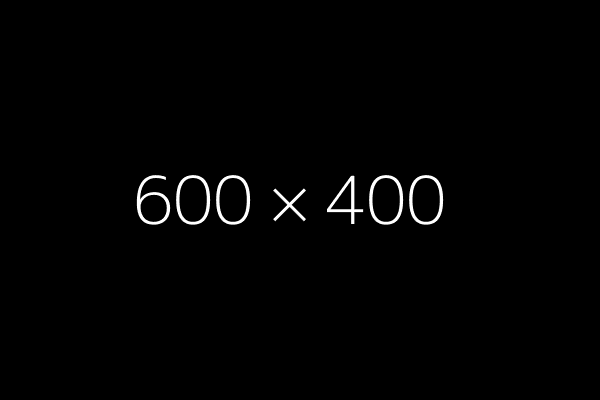
\includegraphics[width=0.6\textwidth]{chapter3/image}
\caption[Short caption for List of Figures]{{\bfseries Short caption (if wanted).} Full caption with all the details here.}\label{fig:1}
\end{figure}
Figures must be accompanied by a caption that describes the material clearly and succinctly.
Figure captions may start with a brief title in bold, which can then be referenced in the list of figures.

Figures should not have captions that run across pages, as a general rule.
If a figure and its caption will be larger than a page, consider rewriting the caption, or reorganizing the figure.
If this cannot be avoided, the figure caption should continue on the immediate next page, with a reference comment at the start of the text to the fact that it is a continuation of the caption from the previous page.
No other main body text should then appear on that page.
\section{Tables}

\begin{table}
\center%
\caption{Short heading for the List of Tables.}
\begin{tabular}{c c}
Parameter & Value \\ \midrule \midrule
$\Delta$ & 0, 150 \\
${\alpha}$ & 85 \\
${\epsilon}$ & 6 \\
${\kappa}$ & 6.8 \\
${\gamma}$ & 0.2
\end{tabular}\label{tab:1}
\caption*{Full caption with all the details here.}
\end{table}

\begin{table} \center%
\begin{tabular}{c c}
Parameter & Value \\ \midrule \midrule
$\Delta$ & 0, 1500 \\
${\alpha}$ & 850 \\
${\epsilon}$ & 60 \\
${\kappa}$ & 68 \\
${\gamma}$ & 2
\end{tabular}\label{tab:2}
\caption*{This secret table won't be numbered and won't appear in the List of Figures because of the * }
\end{table}

All tables should be referred to in the text by number (for example) “Table~\ref{tab:1} describes all particles found in \ldots''.
Tables may be printed in landscape mode rather than portrait mode, but must then be printed on a separate page (with continuing and sequential pagination).
Tables may extend for more than one page, but should then have the table header row repeated on each page.
Do not use font sizes smaller than 9 point.
Tables should have a heading and may have a caption.
The number of the chapter should be part of the Table number.